\documentclass[10pt]{report}
\usepackage[utf8]{inputenc}
\usepackage[greek]{babel}
\usepackage{tikz} 
\usepackage{listings}
\newcommand{\en}{\selectlanguage{english}}
\newcommand{\gr}{\selectlanguage{greek}}
\usepackage{fancyhdr}
\pagestyle{plain}
\fancyhf{}
\fancyhead[R]{\leftmark \gr ΛΕΚΚΑΣ ΓΕΩΡΓΙΟΣ ΑΜ:1067430}
\fancyhead[LO]{\rightmark }
\fancypagestyle{plain}{}
\usepackage{graphicx}
\usepackage{amsthm}

\title{\textbf{1o  {\en PROJECT} ΑΠΟΚΕΝΤΡΩΜΕΝΟΣ ΥΠΟΛΟΓΙΣΜΟΣ \& ΜΟΝΤΕΛΟΠΟΙΗΣΗ}}
\author{\gr ΛΕΚΚΑΣ ΓΕΩΡΓΙΟΣ ΑΜ:1067430  Έτος 5ο\newline}
\date{}
\cfoot{\thepage}
\begin{document}
	\maketitle	
	\thispagestyle{fancy}
	\tableofcontents
	\pagestyle{plain}
	\begin{itemize}
		\item[A.] \gr Άσκηση 1 
		\item[Β.] \gr Άσκηση 2
		
	\end{itemize}
	\pagebreak
	\gr Η συγγραφή της αναφοράς πραγματοποιήθηκε σε {\en Latex} με τη βοήθεια του {\en TexStudio}.\\ \\ 
	\section*{\gr \textbf{Α. Άσκηση 1}}
	\subsection*{\gr Ερώτημα 1}
	\gr Γνωρίζουμε πως σε ένα {\en Randomized} αλγόριθμο υπάρχουν τέσσερις πιθανές ιδιότητες που μπορεί να έχει ένας κόμβος.Μπορεί 1) να είναι {\en Running}, δηλαδή να μην έχει σταθεροποιηθεί το χρώμα του, 2) να είναι {\en Stopped}, δηλαδή να έχει κάποιο χρώμα, 3) να είναι ενεργός, δηλαδή αυτό το γύρο θα προσπαθήσει να βρει χρώμα και 4) να είναι ανενεργός. Επιπλέον σύκρουση κόμβων πραγματοποιείται οταν δύο γειτονικοί κόμβοι έχουν το ίδιο χρώμα(Η έννοια αυτή χρησιμοποιείται στις παρακάτω αποδείξεις).
	
	
	\par \gr Στο πρώτο ερώτημα της άσκησης επιθυμούμε ο κόμβος να ενεργοποιείται με πιθανότητα {\en p{\scriptsize a}}. Συνεπώς η ανάλυση η ανάλυση για αυτόν τον αλγόριθμο όταν η πιθανότητα ενεργοποίησης είναι {\en p{\scriptsize a}} είναι η ακόλουθη:\\
	\par Έστω ότι έχουμε ένα κόμβο {\en u} ο οποίος είναι {\en running} και έχει ως γείτονες {\en k running} κόμβους {\en v}.\\ Τώρα ας υποθέσουμε πως ο {\en u} είναι ενεργός και έχει τουλάχιστον {\en k}+1 διαθέσιμα χρώματα. Τότε {\en A{\scriptsize ri}} είναι η πιθανότητα ο {\en u} να συγκρουστεί με τον {\en v{\scriptsize i}}: $\frac{1}{{\en k}+1}$. Δηλαδή {\en P{\scriptsize r}}({\en A{\scriptsize ri}}) $\leq$$\frac{1}{{\en k}+1}$ (Φράζουμε διότι μπορεί να έχω παραπάνω χρώματα).Άμα ο {\en vi} είναι ανενεργός τότε δεν υπάρχει σύγκρουση.\\Συνεπώς ισχύει το παρακάτω :{\en P{\scriptsize r}}({\en A{\scriptsize ri}}/{\scriptsize {\en vi} ενεργός}) $\leq$$\frac{1}{{\en k}+1}$.\\
	\par Άμα {\en v{\scriptsize i}} ενεργός με πιθανότητα {\en p{\scriptsize a}} τότε: {\en P{\scriptsize r}}({\en A{{\en v{\scriptsize i}}}) $\leq$p{\scriptsize a}/{\en k}+1.\gr Γενικά θέλω να υπολογίσω : {\en P{\scriptsize r}}({\en A{{\en v{\scriptsize 1}}}}$\cup${\en A{{\en v{\scriptsize 2}}}}$\cup${\en A{{\en v{\scriptsize 3}}}}$\cup$...$\cup${\en A{{\en v{\scriptsize k}}}}). Οπότε εφαρμόζω {\en Union Bound} και έχω: {\en P{\scriptsize r}}({\en A{{\en v{\scriptsize 1}}}}$\cup${\en A{{\en v{\scriptsize 2}}}}$\cup${\en A{{\en v{\scriptsize 3}}}}$\cup$...$\cup${\en A{{\en v{\scriptsize k}}}})$\leq$$\sum_{n=1}^{10}${\en P{\scriptsize r}}({\en A{{\en v{\scriptsize i}}}))$\leq${\en k$\cdot$p{\scriptsize a}}/{\en k}+1$\leq${\en k$\cdot$p{\scriptsize a}}/{\en k}$\leq$p{\scriptsize a}}.\\
	Συνεχίζοντας η πιθανότητα να μην συγκρουστούν οι δύο κόμβοι είναι:\\ {\en P{\scriptsize r}}(1/{\en A{{\en v{\scriptsize 1}}}}$\cup${\en A{{\en v{\scriptsize 2}}}}$\cup${\en A{{\en v{\scriptsize 3}}}}$\cup$...$\cup${\en A{{\en v{\scriptsize k}}}}) = 1-{\en P{\scriptsize r}}({\en A{{\en v{\scriptsize 1}}}}$\cup${\en A{{\en v{\scriptsize 2}}}}$\cup${\en A{{\en v{\scriptsize 3}}}}$\cup$...$\cup${\en A{{\en v{\scriptsize k}}}})$\geq${\en p{\scriptsize a}}.\\
	Άρα {\en P{\scriptsize r}}({\en u} να μην συγκρουστεί και να σταματήσει και να πάρει χρώμα)$\geq${\en p{\scriptsize a}}$\cdot${\en p{\scriptsize a}}$\geq${\en p{\scriptsize a}}$^2$.\\
	\par Βασιζόμενοι στο {\en Lemma} της διαφάνειας 61 του δευτερου σετ διαφανειών έχουμε: {\en P{\scriptsize r}}(να μην σταματήσει)$\leq$1-{\en p{\scriptsize a}}$^2$. Συνεπώς η πιθανότητα να μην σταματήσει σε Τ γύρους είναι: (1-{\en p{\scriptsize a}}$^2$)$\cdot$(1-{\en p{\scriptsize a}}$^2$)$\cdot$...(Τ φορές)$\leq$(1-{\en p{\scriptsize a}}$^2$)$^{\en T}$.
	\par Τέλος για να καταλήξω στο δεύτερο {\en Corollary} της διαφάνειας 61 του δευτερου σετ διαφανειών πρέπει αρχικα να καθορίσω το Τ=Ο($\log_{}{\en n}$).Πρέπει δηλαδή να ορίσω τις σταθερές που κρύβει το Ο.Έχουμε: Τ={\en c}$\cdot$$\log_{\frac{1}{1-{\en p{\scriptsize a}}^2}}{\en n}$. Οπότε ένας κόμβος θα σταματήσει με πιθανότητα $\leq(\frac{1}{\frac{1}{1-{\en p{\scriptsize a}}^2}})^{{\en c}\cdot\log_{\frac{1}{1-{\en p{\scriptsize a}}^2}}{\en n}}\leq(\frac{1}{1-{\en p{\scriptsize a}}^2})^{-1\cdot{\en c}\cdot\log_{\frac{1}{1-{\en p{\scriptsize a}}^2}}{\en n}}\leq{\en n}^{\en -c}$.\\
	Aπό {\en Union Bound} έχουμε : {\en P{\scriptsize r}}(να μην έχει τελίωσει κάποιος κόμβος μετά από Τ γύρους)$\leq{\en n}\cdot{\en n}^{\en -c}={\en n}^{\en -c+1}$. Οπότε η πιθανότητα να μην έχει τερματίσει κάποιος κόμβος μετά από {\en c}$\cdot$$\log_{\frac{1}{1-{\en p{\scriptsize a}}^2}}{\en n}$ γύρους είναι το πολύ $\frac{1}{{\en n}^{\en c-1}}$. Συμπερασματικά, η πιθανότητα να τερματίσει μετά από {\en c}$\cdot$$\log_{\frac{1}{1-{\en p{\scriptsize a}}^2}}{\en n}$ γύρους είναι $\leq 1-\frac{1}{{\en n}^{\en c-1}}$ ,δηλαδή {\en w.h.p}.\\															
																								\qed
	\subsection*{\gr Ερώτημα 2}
	\gr Όταν {\en p{\scriptsize a}}=1 δηλαδή όταν η παράμετρος που δηλώνει την πιθανότητα ενεργοποίησης  ενός κόμβου είναι ίση με 1, αυτό σημαίνει πως όλοι οι κόμβοι ψάχνουν να βρουν ένα διαθέσιμο χρώμα.\\
	Από την απόδειξη του προηγούμενου ερωτήματος συνεχίζουμε από το σημείο υπολογισμού του {\en P{\scriptsize r}}({\en A{{\en v{\scriptsize i}}}}) και έχουμε: {\en P{\scriptsize r}}({\en A{{\en v{\scriptsize i}}}})$\leq\frac{1}{{\en k}+1}$.\\
	Οπότε εφαρμόζω {\en Union Bound} και έχω: {\en P{\scriptsize r}}({\en A{{\en v{\scriptsize 1}}}}$\cup${\en A{{\en v{\scriptsize 2}}}}$\cup${\en A{{\en v{\scriptsize 3}}}}$\cup$...$\cup${\en A{{\en v{\scriptsize k}}}})$\leq$$\sum_{n=1}^{10}${\en P{\scriptsize r}}({\en A{{\en v{\scriptsize i}}}))\\$\leq$$\frac{\en k}{{\en k}+1}$$\leq$$\frac{\en k}{{\en k}}$$\leq$1.\\
	\gr Συνεχίζοντας η πιθανότητα να μην συγκρουστούν οι δύο κόμβοι είναι:\\ {\en P{\scriptsize r}}(1/{\en A{{\en v{\scriptsize 1}}}}$\cup${\en A{{\en v{\scriptsize 2}}}}$\cup${\en A{{\en v{\scriptsize 3}}}}$\cup$...$\cup${\en A{{\en v{\scriptsize k}}}}) = 1-{\en P{\scriptsize r}}({\en A{{\en v{\scriptsize 1}}}}$\cup${\en A{{\en v{\scriptsize 2}}}}$\cup${\en A{{\en v{\scriptsize 3}}}}$\cup$...$\cup${\en A{{\en v{\scriptsize k}}}})$\geq$0(Οριακά μεγαλύτερη ή ίση του μηδενός).\\
	Συνεπώς θα υπάρχει  σχεδόν πάντα σύγκρουση μεταξύ δύο γειτονικών κόμβων.\\ Δηλαδή δεν θα μπορέσουν να πάρουν  σχεδόν ποτέ χρώμα το οποίο να συμβαδίζει με τους κανόνες χρωματισμού.Η αποδοτικότητα του συγκεκριμένου αλγορίθμου είναι πάρα πολυ μικρή. \\ \\
	
	\gr Για να είναι ο αλγόριθμος αποδοτικός θα πρέπει να μειωθεί ο αριθμός των χρωμάτων σημαντικά διότι έτσι αποφεύγουμε περισσότερες συγκρούσεις,αφού λιγότεροι κόμβοι θα έχουν ίδιο χρώμα με τους γείτονές τους.
																								
	\pagebreak																								
	\section*{\gr \textbf{Β. Άσκηση 2}}	
	
	\gr \large{Περιγραφή αλγορίθμου:}\\
	
	\gr \normalsize Σύμφωνα με τις διαφάνειες ο γρήγορος αλγόριθμος για χρωματισμό καταφέρνει μετά από $\log_{}^*{{\en n}}$ γύρους να περιορίσει τον αριθμό των χρωμάτων από {\en x} σε 6.Βασιζόμενοι στον παραπάνω αλγόριθμο και στο γεγονός ότι σε κάθε γύρο μειώνει τον αριθμό των χρωμάτων από {\en x} σε Ο($\log_{}{{\en x}}$) τότε μπορούμε να περιγράψουμε τον παρακάτω αλγόριθμο :\\ \\
	Έστω ότι έχουμε 6 χρώματα (0,1,2,3,4,5).\\
	Αρχικά ορίζουμε υπορουτίνα η οποία θα χρησιμοποιηθεί για να διατηρείται η αρχή του χρωματισμού των γειτονικών κόμβων.Δηλαδή ότι δεν πρέπει γειτονικοί κόμβοι να έχουν το ίδιο χρώμα.\\
	Υπορουτίνα: 
	\begin{enumerate}
		\item Η ρίζα επιλέγει ένα χρώμα από τα {0,1,2}.
		\item Κάθε κόμβος ξαναχρωματίζεται με το χρώμα που είχε ο γονιός του.
	\end{enumerate}
	 
	Αλγόριθμος:\\
	Κάθε κόμβος σε παράλληλο χρόνο:      
	\begin{enumerate}
		\item Τρέχει τον γρήγορο αλγόριθμο χρωματισμού μέχρι να φτάσει στα 6 χρώματα.
		\item Για {\en x} =5,4,3:
		\begin{enumerate}
			\item Eκτελεί την υπορουτίνα που αναφέρθηκε παραπάνω.
			\item Αν το χρώμα ενός κόμβου μετά την υπορουτίνα είναι 5 ή 4 ή 3 τότε επιλέγεται το μικρότερο και ελεύθερο νέο χρώμα από το {0,1,2} .
		\end{enumerate} 
	\end{enumerate}
	Αυτό το {\en loop} συνεχίζεται μέχρι να καταλήξουμε σε έναν αποδεκτό χρωματισμό του δένδρου που θα περιλαμβάνει μόνο 3 χρώματα χωρίς την ύπαρξη {\en adjacent} κόμβων.\\ \\ \\
	
	Στην συνέχεια παρουσιάζεται μια πιθανή εκτέλεση του παραπάνω αλγορίθμου:\\ \\
	
	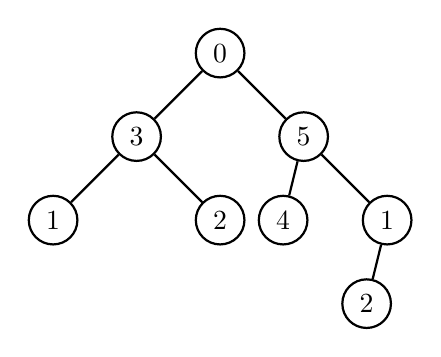
\begin{tikzpicture}[node distance={15mm}, thick, main/.style = {draw, circle}] 
		\node[main] (1) {$0$};
		\node[main] (2) [below left of=1] {$3$};	
		\node[main] (3) [below right of=1] {$5$};
		\node[main] (4) [below left of=2] {$1$};
		\node[main] (5) [below right of=2] {$2$};
		\node[main,xshift = 0.8cm] (6) [below left of=3] {$4$};
		\node[main] (7) [below right of=3] {$1$};
		\node[main] (8) [below right of=6] {$2$};
		
		\draw (1) -- (2);
		\draw (1) -- (3);
		\draw (2) -- (4);
		\draw (2) -- (5); 
		\draw (3) -- (6);
		\draw (3) -- (7);
		\draw (7) -- (8);
	\end{tikzpicture}

	\pagebreak
	Μετά την υπορουτίνα:\\
	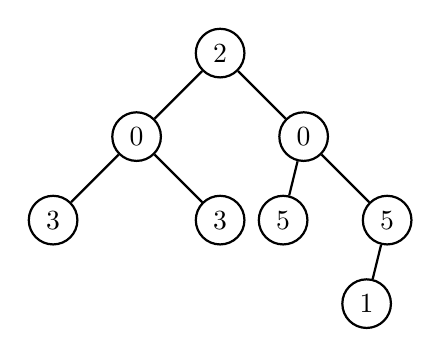
\begin{tikzpicture}[node distance={15mm}, thick, main/.style = {draw, circle}] 
		\node[main] (1) {$2$};
		\node[main] (2) [below left of=1] {$0$};	
		\node[main] (3) [below right of=1] {$0$};
		\node[main] (4) [below left of=2] {$3$};
		\node[main] (5) [below right of=2] {$3$};
		\node[main,xshift = 0.8cm] (6) [below left of=3] {$5$};
		\node[main] (7) [below right of=3] {$5$};
		\node[main] (8) [below right of=6] {$1$};
		
		\draw (1) -- (2);
		\draw (1) -- (3);
		\draw (2) -- (4);
		\draw (2) -- (5); 
		\draw (3) -- (6);
		\draw (3) -- (7);
		\draw (7) -- (8);
	\end{tikzpicture}

	Μετά το βήμα 2 του {\en for loop}:\\
	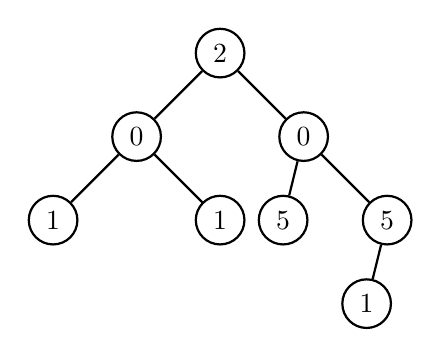
\begin{tikzpicture}[node distance={15mm}, thick, main/.style = {draw, circle}] 
		\node[main] (1) {$2$};
		\node[main] (2) [below left of=1] {$0$};	
		\node[main] (3) [below right of=1] {$0$};
		\node[main] (4) [below left of=2] {$1$};
		\node[main] (5) [below right of=2] {$1$};
		\node[main,xshift = 0.8cm] (6) [below left of=3] {$5$};
		\node[main] (7) [below right of=3] {$5$};
		\node[main] (8) [below right of=6] {$1$};
		
		\draw (1) -- (2);
		\draw (1) -- (3);
		\draw (2) -- (4);
		\draw (2) -- (5); 
		\draw (3) -- (6);
		\draw (3) -- (7);
		\draw (7) -- (8);
	\end{tikzpicture}

		Μετά την υπορουτίνα:\\
	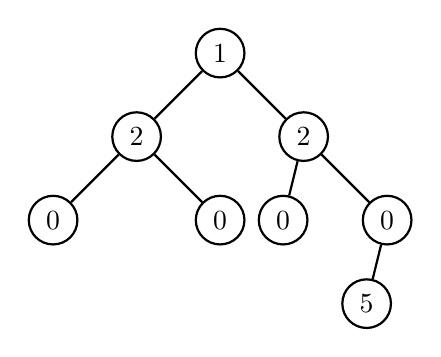
\begin{tikzpicture}[node distance={15mm}, thick, main/.style = {draw, circle}] 
		\node[main] (1) {$1$};
		\node[main] (2) [below left of=1] {$2$};	
		\node[main] (3) [below right of=1] {$2$};
		\node[main] (4) [below left of=2] {$0$};
		\node[main] (5) [below right of=2] {$0$};
		\node[main,xshift = 0.8cm] (6) [below left of=3] {$0$};
		\node[main] (7) [below right of=3] {$0$};
		\node[main] (8) [below right of=6] {$5$};
		
		\draw (1) -- (2);
		\draw (1) -- (3);
		\draw (2) -- (4);
		\draw (2) -- (5); 
		\draw (3) -- (6);
		\draw (3) -- (7);
		\draw (7) -- (8);
	\end{tikzpicture}
	
	Μετά το βήμα 2 του {\en for loop}:\\
	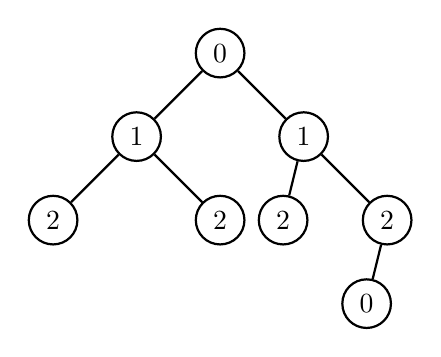
\begin{tikzpicture}[node distance={15mm}, thick, main/.style = {draw, circle}] 
		\node[main] (1) {$0$};
		\node[main] (2) [below left of=1] {$1$};	
		\node[main] (3) [below right of=1] {$1$};
		\node[main] (4) [below left of=2] {$2$};
		\node[main] (5) [below right of=2] {$2$};
		\node[main,xshift = 0.8cm] (6) [below left of=3] {$2$};
		\node[main] (7) [below right of=3] {$2$};
		\node[main] (8) [below right of=6] {$0$};
		
		\draw (1) -- (2);
		\draw (1) -- (3);
		\draw (2) -- (4);
		\draw (2) -- (5); 
		\draw (3) -- (6);
		\draw (3) -- (7);
		\draw (7) -- (8);
	\end{tikzpicture}
	
	

	
	
		
		
		
		
\end{document}